\documentclass[mathserif, handout]{beamer}

\usepackage{url}
% ======================================================================
% General LaTeX Setup for Beamer (Reusable Preamble)
% Author: Chandra Gummaluru
% ======================================================================

\documentclass[mathserif, handout]{beamer}
\setbeamertemplate{frametitle}{}

% ------------------------------------------------------------
% basic packages
% ------------------------------------------------------------
\usepackage{url}
\usepackage{ifthen}
\usepackage{enumerate}
\usepackage[font=small]{caption}
\usepackage{subcaption}
\usepackage{moresize}
\usepackage[outline]{contour}
\usepackage{transparent}
\usepackage{worldflags}
\usepackage{bm}
\usepackage{graphbox}
\usepackage{mathtools}
\usepackage{multirow}
\usepackage{fontawesome5}
\usepackage{pifont}
\usepackage{array}
\usepackage{comment}

% ------------------------------------------------------------
% math
% ------------------------------------------------------------
\DeclarePairedDelimiter{\floor}{\lfloor}{\rfloor}
\DeclarePairedDelimiter{\ceil}{\lceil}{\rceil}

% ------------------------------------------------------------
% colors
% ------------------------------------------------------------
\definecolor{hl}{RGB}{248,196,69}
\definecolor{myred}{HTML}{ED5565}
\definecolor{myorange}{HTML}{FC6E51}
\definecolor{myyellow}{HTML}{FFCE54}
\definecolor{mycyan}{HTML}{4FC1E9}
\definecolor{myblue}{HTML}{5D9CEC}

\newcommand{\graytext}[1]{\footnotesize\color{gray}#1\normalsize\color{black}}

% ------------------------------------------------------------
% symbols
% ------------------------------------------------------------
\newcommand{\cmark}{\ding{51}}
\newcommand{\xmark}{\ding{55}}

% ------------------------------------------------------------
% highlighting
% ------------------------------------------------------------
\newcommand{\reducedstrut}{\vrule width 0pt height .9\ht\strutbox depth .9\dp\strutbox\relax}
\newcommand{\highlight}[1]{%
  \begingroup\setlength{\fboxsep}{0pt}\colorbox{hl}{\reducedstrut$\displaystyle #1$\/}\endgroup}
\newcommand{\highlightc}[2]{%
  \begingroup\setlength{\fboxsep}{0pt}\colorbox{#1}{\reducedstrut$\displaystyle #2$\/}\endgroup}

% ------------------------------------------------------------
% environments (boxes)
% ------------------------------------------------------------
\usepackage{tcolorbox}
\tcbuselibrary{skins}

\newtcolorbox{thmbox}[1][]{colback=gray!30!white!20, colframe=black, fonttitle=\bfseries, title=#1, boxrule=0.5pt}

% 1) Bottom open (draw top + sides only)
\newtcolorbox{thmboxtop}[1][]{
    enhanced,
    frame hidden,
    colback=gray!30!white!20,
    borderline north={0.5pt}{0pt}{black}, % top
    borderline west={0.5pt}{0pt}{black},  % left
    borderline east={0.5pt}{0pt}{black}   % right
}

% 2) Top open (draw bottom + sides only)
\newtcolorbox{thmboxbot}[1][]{
    enhanced,
    frame hidden,
    colback=gray!30!white!20,
    borderline south={0.5pt}{0pt}{black}, % bottom
    borderline west={0.5pt}{0pt}{black},  % left
    borderline east={0.5pt}{0pt}{black}   % right
}

% 3) Side only (draw only left and right)
\newtcolorbox{thmboxside}[1][]{
    enhanced,
    frame hidden,
    colback=gray!30!white!20,
    borderline west={0.5pt}{0pt}{black},  % left
    borderline east={0.5pt}{0pt}{black}   % right
}

\newtcolorbox{defboxtop}[1][]{
    enhanced,
    colback=gray!30!white!20,
    frame hidden,
    overlay={
        % Draw top + sides with rounded corners
        \draw[line width=0.5pt, black, rounded corners=3mm]
            (frame.south west) -- (frame.north west) -- (frame.north east) -- (frame.south east);
    },
    #1
}

\newtcolorbox{defboxbot}[1][]{
    enhanced,
    colback=gray!30!white!20,
    frame hidden,
    overlay={
        % Draw top + sides with rounded corners
        \draw[line width=0.5pt, black, rounded corners=3mm]
            (frame.north west) -- (frame.south west) -- (frame.south east) -- (frame.north east);
    },
    #1
}

\newtcolorbox{defboxside}[1][]{
    enhanced,
    frame hidden,
    colback=gray!30!white!20,
    borderline west={0.5pt}{0pt}{black},  % left
    borderline east={0.5pt}{0pt}{black}   % right
}

\newtcolorbox{proofbox}[1][]{colback=gray!20!white!20, colframe=grey, fonttitle=\bfseries, title=#1, boxrule=0.5pt, colbacktitle=white, enhanced jigsaw, sharp corners}

% ------------------------------------------------------------
% code listings
% ------------------------------------------------------------
\usepackage{listings}
\lstdefinestyle{mypython}{
  language=Python,
  deletekeywords=[2]{open, next, from, chr, str, int},
  morekeywords=[3]{List, Graph, Tree, Dict, Set, UnionFind, Ordict, Trie, Queue},
  morekeywords=[4]{ListNode, Vertex, Edge, Path, TreeNode, DictNode, UnifNode, OrdictNode, TrieNode, QueueNode},
  morekeywords=[5]{True, False, Boolean, String, Integer, Key, Function, KeyedObject, Object, Array, Tuple, Optional, None},
  keywordstyle=\color{mycyan}\bfseries,
  keywordstyle=[3]\color{myblue}\bfseries,
keywordstyle=[4]\color{myblue}\bfseries,
keywordstyle=[5]\color{mycyan}\bfseries,
  stringstyle=\color{orange},
  commentstyle=\color{gray}\itshape,
  basicstyle=\ttfamily\footnotesize,
  numbers=left,
  numberstyle=\tiny\color{gray},
  stepnumber=1,
  numbersep=5pt,
  xleftmargin=15pt,
  frame=none,
  showstringspaces=false,
  breaklines=true,
  breakatwhitespace=true,
  tabsize=4,
  columns=flexible
}


% ------------------------------------------------------------
% algorithms
% ------------------------------------------------------------
\usepackage{algorithm}
\usepackage[endLComment=~]{algpseudocodex}
\makeatletter
\algrenewcommand\ALG@beginalgorithmic{\footnotesize}
\makeatother

% ------------------------------------------------------------
% optimization environments
% ------------------------------------------------------------
\usepackage[nocomma]{optidef}

% ------------------------------------------------------------
% pgfplots and pie charts
% ------------------------------------------------------------
\usepackage{pgfplots}
\usepackage{pgf-pie}
\pgfplotsset{compat=1.7}

% ------------------------------------------------------------
% tikz
% ------------------------------------------------------------
\usepackage{tikz}
\usetikzlibrary{
  angles, quotes, positioning, fit, backgrounds, shapes.geometric, intersections,
  calc, shapes, mindmap, decorations.text, arrows, arrows.meta,
  automata, chains, decorations.pathreplacing, calligraphy,
  decorations.markings, shapes.misc, decorations.pathmorphing
}
\tikzset{
  invisible/.style={opacity=0},
  visible on/.style={alt=#1{}{invisible}},
  alt/.code args={<#1>#2#3}{\alt<#1>{\pgfprioritysalso{#2}}{\pgfprioritysalso{#3}}}
}

\newcommand{\multiedge}[5][]{
\pgfmathsetmacro{\N}{#4}
\pgfmathsetmacro{\mid}{(\N-1)/2}
\foreach \i in {0,...,\numexpr#4-1\relax} {

\pgfmathsetmacro{\k}{\i-\mid}
\draw[#1] ($ (#2) + \k*#5*($(#2)!1!90:(#3)$) $) -- ($ (#3) + \k*#5*($(#2)!1!90:(#3)$) $); 

}
\draw[#1,  -{>[scale=1]}]
  ($(#2)!0.54!(#3)$) -- ($(#2)!0.55!(#3)$);
}

% ------------------------------------------------------------
% bibliography
% ------------------------------------------------------------
\usepackage[style=ieee]{biblatex}
\setbeamertemplate{bibliography item}{\insertbiblabel}
\setbeamertemplate{background canvas}{
  \begin{tikzpicture}[remember picture,overlay]
    \node[opacity=0.0075]
      at (current page.center)
      {
\includegraphics[width=0.8\paperwidth]{images/signature.pdf}};
  \end{tikzpicture}
}

% ------------------------------------------------------------
% beamer theme and settings
% ------------------------------------------------------------
\usetheme{Boadilla}
\usecolortheme{seagull}
\beamertemplatenavigationsymbolsempty
\setbeamertemplate{enumerate item}{(\arabic{enumi})}
\setbeamertemplate{enumerate subitem}{(\alph{enumii})}
\setbeamertemplate{enumerate subsubitem}{(\roman{enumiii})}
\setbeamertemplate{itemize item}[circle]
\setbeamertemplate{itemize subitem}{\circ}
\setbeamertemplate{itemize subsubitem}{-}
\setbeamercolor{item}{fg=black!40}
\setbeamercovered{transparent=10}

% ===========================
% Premade TikZ Figure Commands
% ===========================

% images w/ labels
% inside tikz as a node
\NewDocumentCommand{\labeledimgnodetikz}{O{} m m m m m m}{%
	\begin{scope}[transparency group, #1]
		\node[
			draw,
			circle,
			inner sep=0,
			outer sep=0,
			minimum size=10mm,
			#1
		] (#5) at (#3,#4)
		{\includegraphics[scale=#7]{#6}};
		\node[
			rectangle,
			draw=black,
			thick,
			fill=black!55,
			rounded corners=0.1mm,
			inner sep=0pt,
			outer sep=0pt,
			minimum size=2.8mm,
			minimum width=3.5mm
		] at (#3,#4-0.1) {};
		\node[outer sep=0, inner sep=0, white] at (#3,#4-0.1) {\footnotesize #2};
	\end{scope}
}

% inside tikz isolated

% outside tikz
\NewDocumentCommand{\labelednode}{m}{%
	\begin{tikzpicture}[baseline={(0,-1mm)}]
		\node[
			rectangle,
			thick,
			draw=black,
			fill=black!55,
			rounded corners=0.1mm,
			inner sep=0pt,
			outer sep=0pt,
			minimum size=2.8mm,
			minimum width=3.5mm
		] at (0,0) {};
		\node[outer sep=0, inner sep=0, white, minimum size=2.8mm, minimum width=3.5mm] at (0,0) {\footnotesize #1};
	\end{tikzpicture}
}

% images only
% inside tikz as a node
\NewDocumentCommand{\imgnodetikz}{O{} m m m m m m}{%
	\begin{scope}[transparency group, #1]
		\node[
			draw,
			circle,
			inner sep=0,
			outer sep=0,
			minimum size=10mm,
			#1
		] (#5) at (#3,#4)
		{\includegraphics[scale=#7]{#6}};
		\node[
			rectangle,
			draw,
			thick,
			fill=black!55,
			rounded corners=0.1mm,
			inner sep=0pt,
			outer sep=0pt,
			minimum size=2.8mm,
			minimum width=3.5mm,
			opacity=0
		] at (0,0) {};
		\node[outer sep=0, inner sep=0, white, opacity=0] at (0,0) {\footnotesize #2};
	\end{scope}
}

% inside tikz isolated
\NewDocumentCommand{\imgtikz}{O{} mm}{%
	\begin{scope}[transparency group, #1]
		\node[
			inner sep=0,
			outer sep=0
		] (#5) at (#3,#4)
		{\includegraphics[scale=#3]{#2}};
	\end{scope}
}


% outside tikz
\NewDocumentCommand{\imgnode}{mm}{%
	\begin{tikzpicture}[baseline={(0,-1mm)}]
        \node[
            inner sep=0,
            outer sep=0,
            draw opacity=0,
        ] at (0,0)
        {\includegraphics[scale=#2]{#1}};
    \end{tikzpicture}
}

% outside tikz (inline)
\newcommand{\imgnodetext}[2]{%
	\hspace{-0.5mm}%
	\raisebox{-0.26\height}{%
		\includegraphics[scale=#2]{#1}%
	}%
	\hspace{-0.5mm}%
}


% labels only
% inside tikz as a node
\NewDocumentCommand{\labeltikz}{m}{%
	\node[
		rectangle,
		thick,
		draw=black,
		fill=black!55,
		rounded corners=0.1mm,
		inner sep=0pt,
		outer sep=0pt,
		minimum size=2.8mm,
		minimum width=3.5mm
	] at (0,0) {};
	\node[outer sep=0, inner sep=0, white, draw opacity=0] at (0,0) {\footnotesize #1};
}

% inside tikz isolated

% outside tikz

% === define custom pgfkeys ===
\pgfkeys{
	/devicenode/.is family, /devicenode,
	outline thickness/.initial=thick,
	outline color/.initial=black
}

\NewDocumentCommand{\qpacket}{m}{%
	\begin{tikzpicture}[baseline=(current bounding box.center)]
		\node at (0.5,0.4) {\includegraphics[scale=0.1]{#1}};
	\end{tikzpicture}%
}

\NewDocumentCommand{\bpacketid}{mmm}{%
	\begin{tikzpicture}[baseline=(current bounding box.center)]
		\begin{scope}[shift={(0.85,0.7)}]
			\draw[thick, draw=black, fill=#1, rounded corners=1pt] (0.01,0.05) rectangle node[white, text width=1cm, align=center] {\color{#3}\footnotesize #2} (-0.71,-0.625);
		\end{scope}
	\end{tikzpicture}%
}

\NewDocumentCommand{\packetid}{mmmm}{%
	\begin{tikzpicture}[baseline=(current bounding box.center)]
		\begin{scope}[shift={(0.85,0.7)}]
			\draw[thick, draw=black, fill=#2, rounded corners=1pt] (0.01,0.05) rectangle node[white, text width=1cm, align=center] {\color{#4}\footnotesize #3} (-0.71,-0.625);
			\node[
				star,
				star points=30,
				star point ratio=0,
				scale=1.5,
				draw=black,
				thick,
				fill=white,
				rounded corners=0.1mm,
				inner sep=0pt,
				minimum size=2.8mm
			] at (0,0) {};
			\node at (0,0) {\footnotesize #1};
		\end{scope}
	\end{tikzpicture}%
}

\tikzset{
	dictnode/.pic={
			\draw[thick, fill=#1, line join=]
			(-0.75,-0.5) --
			(-0.75,0.5)  --
			(0.75,0.5) --
			(0.75,-0.5) --
			cycle --
			(-0.75, 0.75) --
			(0.75, 0.75) --
			(0.75, -0.5) --
			cycle;
		}
}

\tikzset{
	queuenode/.pic={
			\draw[thick, fill=#1, line join=round]
			(-0.85,-0.5) --
			(-0.85,0.5)  --
			(0.65,0.5) --
			(0.75,0) --
			(0.65,-0.5) --
			cycle;
		}
}

\tikzset{
	queuenodetail/.pic={
			\draw[thick, fill=#1, line join=round]
			(-0.75,-0.5) --
			(-0.75,0.5)  --
			(0.65,0.5) --
			(0.75,0) --
			(0.65,-0.5) --
			cycle;
		}
}

\tikzset{
	listnode/.style={
			shape=rectangle,
			rounded corners,
			thick,
			minimum height=10mm,
			minimum width=15mm,
			inner sep=0pt
		}
}

\tikzset{
	arraynode/.style={
			shape=rectangle,
			thick,
			minimum height=10mm,
			minimum width=15mm,
			inner sep=0pt
		}
}

\tikzset{
	graphnode/.style={
			shape=circle,
			thick,
			minimum size=5mm,
			inner sep=0pt
		}
}

\tikzset{
	defaultnode/.style={
			transform shape,
			circle,
			draw=black,
			thick,
			fill=white,
			minimum size=10mm,
			inner sep=0pt
		},
	newnode/.style={
			transform shape,
			defaultnode,
			draw=myyellow,
			fill=myyellow!60,
			very thick
		},
	newnodelight/.style={
			transform shape,
			defaultnode,
			draw=myyellow,
			fill=myyellow!30,
			very thick
		},
	deletenode/.style={
			defaultnode,
			draw=gray,
			dashed,
			fill=lightgray,
			text=gray,
			very thick
		},
	nooutlinenode/.style={
			defaultnode,
			draw=none,
            draw opacity=0,
			text=black,
			very thick
		},
    nofillnode/.style={
			defaultnode,
			fill=none,
            text=black,
			very thick
		}
}
\tikzset{
	faded/.style={opacity=0.5, text opacity=0.5, transparency group}
}
\tikzset{
	smallgraytext/.style={font=\footnotesize\color{gray}}
}
\tikzset{
	graytext/.style={font=\normalsize\color{gray}}
}
\tikzset{
  squigglearrow/.style={
    very thick,
    lightgray,
    decorate,
    decoration={
      snake,
      amplitude=1.75pt,
      segment length=8pt
    }
  }
}



\usetikzlibrary{shapes.gates.logic.US}

\newcommand{\ttab}[1]{\texttt{#1}}

% title
\title{Logic Devices}
\subtitle{Computer Organization}
\author[C. Gummaluru]{Chandra Gummaluru}
\titlegraphic{
\includegraphics[width=0.15\linewidth]{images/signature.pdf}}
\institute[]{\url{chandra-gummaluru.github.io} }
\date[Computer Organization]{}

\begin{document}

\begin{frame}
  \maketitle
\end{frame}

\begin{frame}
  \begin{center}
    \highlight{\textbf{logic device}} \\[2mm]
    \graytext{a reusable block, built from gates, \\ that performs one common task}
  \end{center}
\end{frame}

\begin{frame}
  We treat each device as a single symbol and reason about what it does, not how its gates are wired.\\[3mm]
  \begin{itemize}
    \item \highlight{\textbf{multiplexer}}\\
    \graytext{selects one input to pass through} \\[2mm]
    \item \highlight{\textbf{decoder}}\\
    \graytext{turns a number into a one-hot signal} \\[2mm]
    \item \highlight{\textbf{encoder}}\\
    \graytext{turns a one-hot signal back into a number}
  \end{itemize}\\[3mm]
These devices give us the vocabulary to describe larger circuits without drawing every gate.
\end{frame}

% ------------------------------------------------------------
% multiplexer
% ------------------------------------------------------------
\begin{frame}{Multiplexer}
  \begin{center}
    \Large \highlight{\textbf{multiplexer}}
  \end{center}
\end{frame}

\begin{frame}
  A \highlight{\textbf{multiplexer}} passes one of its data inputs to the output. A select input chooses which one.\\[3mm]
  \begin{minipage}{0.55\textwidth}
    \centering
    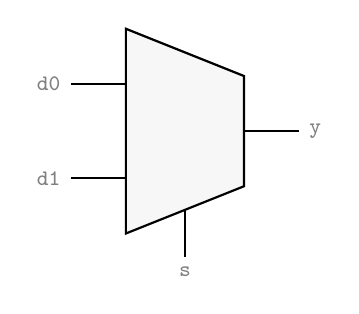
\begin{tikzpicture}
      \draw[thick, fill=gray!30!white!20] (0,1.3) -- (0,-1.3) -- (1.5,-0.7) -- (1.5,0.7) -- cycle;
      \draw[thick] (0,0.6) -- ++(-0.7,0) node[left, smallgraytext] {\ttab{d0}};
      \draw[thick] (0,-0.6) -- ++(-0.7,0) node[left, smallgraytext] {\ttab{d1}};
      \draw[thick] (1.5,0) -- ++(0.7,0) node[right, smallgraytext] {\ttab{y}};
      \draw[thick] (0.75,-1) -- ++(0,-0.6) node[below, smallgraytext] {\ttab{s}};
    \end{tikzpicture}
  \end{minipage}%
  \begin{minipage}{0.45\textwidth}
    \centering
    \renewcommand{\arraystretch}{1.3}
    \begin{tabular}{c|c}
      \ttab{s} & \ttab{y} \\ \hline
      \ttab{0} & \ttab{d0} \\
      \ttab{1} & \ttab{d1} \\
    \end{tabular}
  \end{minipage}
\end{frame}

\begin{frame}
  Inside, the select line either enables one \texttt{AND} gate or the other. Their outputs are combined by an \texttt{OR}.\\[1mm]
  \begin{figure}
    \centering
    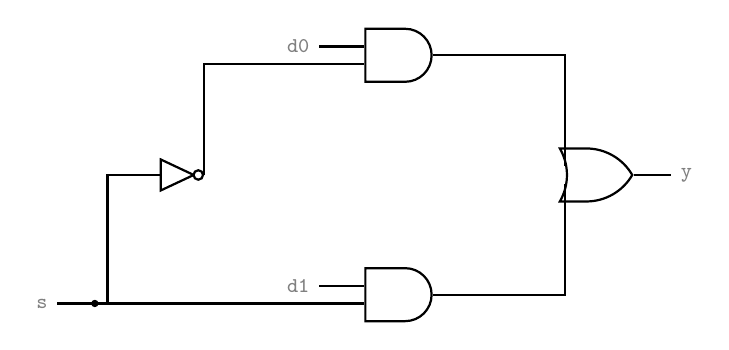
\begin{tikzpicture}[scale=0.95, transform shape]
      \node[and gate US, draw, thick, scale=1.2] (g0) at (0,1.6) {};
      \node[and gate US, draw, thick, scale=1.2] (g1) at (0,-1.6) {};
      \node[or gate US, draw, thick, scale=1.2] (o) at (2.6,0) {};
      \node[not gate US, draw, thick, scale=0.9] (n) at (-3.0,0) {};

      \draw[thick] (g0.input 1) -- ++(-0.6,0) node[left, smallgraytext] {\ttab{d0}};
      \draw[thick] (g1.input 1) -- ++(-0.6,0) node[left, smallgraytext] {\ttab{d1}};

      % NOT gate output feeds g0's second input, routed above g1
      \draw[thick] (n.output) |- (g0.input 2);

      % s branches: one leg into g1's second input, one leg up into the NOT gate
      \draw[thick] (g1.input 2) -- ++(-3.6,0) coordinate (sj);
      \draw[thick] (n.input) -- ++(-0.7,0) |- (sj);
      \draw[thick] (sj) -- ++(-0.5,0) node[left, smallgraytext] {\ttab{s}};
      \fill (sj) circle (1.4pt);

      \draw[thick] (g0.output) -| (o.input 1);
      \draw[thick] (g1.output) -| (o.input 2);
      \draw[thick] (o.output) -- ++(0.5,0) node[right, smallgraytext] {\ttab{y}};
    \end{tikzpicture}
  \end{figure}
  \begin{center}
    \graytext{$\ttab{y} = \overline{\ttab{s}}\cdot \ttab{d0} + \ttab{s} \cdot \ttab{d1}$}
  \end{center}
\end{frame}

\begin{frame}
  With more select inputs, a multiplexer chooses among more data inputs. Two select inputs choose one of four.\\[3mm]
  \begin{center}
    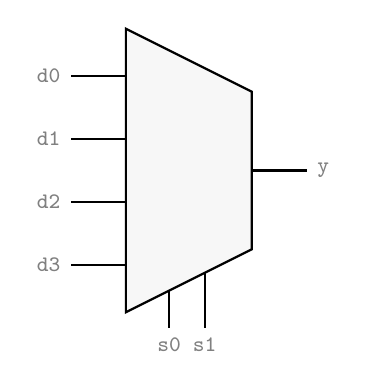
\begin{tikzpicture}
      \draw[thick, fill=gray!30!white!20] (0,1.8) -- (0,-1.8) -- (1.6,-1.0) -- (1.6,1.0) -- cycle;
      \foreach \y/\l in {1.2/d0, 0.4/d1, -0.4/d2, -1.2/d3}
        \draw[thick] (0,\y) -- ++(-0.7,0) node[left, smallgraytext] {\ttab{\l}};
      \draw[thick] (1.6,0) -- ++(0.7,0) node[right, smallgraytext] {\ttab{y}};
      \draw[thick] (0.55,-1.525) -- (0.55,-2.0) node[below, smallgraytext] {\ttab{s0}};
      \draw[thick] (1.0,-1.3) -- (1.0,-2.0) node[below, smallgraytext] {\ttab{s1}};
    \end{tikzpicture}
  \end{center}
  \begin{center}
    \graytext{the select inputs read as a number that picks the data input}
  \end{center}
\end{frame}

\begin{frame}
  A \highlight{\textbf{demultiplexer}} does the reverse. It sends one data input to the one output chosen by the select line.\\[3mm]
  \begin{center}
    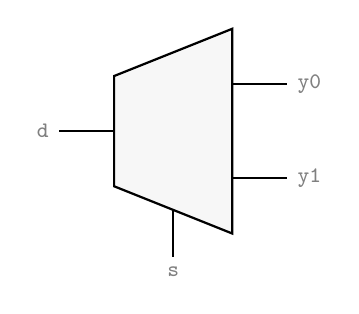
\begin{tikzpicture}
      % mirror-image trapezoid (narrow on the left)
      \draw[thick, fill=gray!30!white!20] (1.5,1.3) -- (1.5,-1.3) -- (0,-0.7) -- (0,0.7) -- cycle;
      \draw[thick] (0,0) -- ++(-0.7,0) node[left, smallgraytext] {\ttab{d}};
      \draw[thick] (1.5,0.6) -- ++(0.7,0) node[right, smallgraytext] {\ttab{y0}};
      \draw[thick] (1.5,-0.6) -- ++(0.7,0) node[right, smallgraytext] {\ttab{y1}};
      \draw[thick] (0.75,-1) -- ++(0,-0.6) node[below, smallgraytext] {\ttab{s}};
    \end{tikzpicture}
  \end{center}
  \begin{center}
    \graytext{a multiplexer merges many lines into one, a demultiplexer splits one into many}
  \end{center}
\end{frame}

% ------------------------------------------------------------
% decoder
% ------------------------------------------------------------
\begin{frame}{Decoder}
  \begin{center}
    \Large \highlight{\textbf{decoder}}
  \end{center}
\end{frame}

\begin{frame}
  A \highlight{\textbf{decoder}} reads its inputs as a number and sets exactly one output to \ttab{1}. This is called a one-hot output.\\[3mm]
  \begin{minipage}{0.45\textwidth}
    \centering
    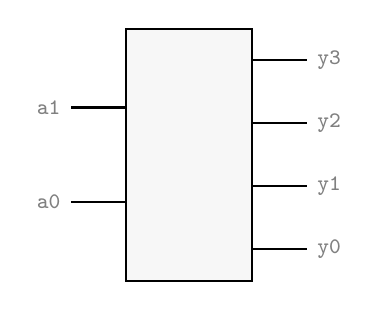
\begin{tikzpicture}
      \draw[thick, fill=gray!30!white!20] (0,-1.6) rectangle (1.6,1.6);
      \draw[thick] (0,0.6) -- ++(-0.7,0) node[left, smallgraytext] {\ttab{a1}};
      \draw[thick] (0,-0.6) -- ++(-0.7,0) node[left, smallgraytext] {\ttab{a0}};
      \foreach \y/\l in {1.2/y3, 0.4/y2, -0.4/y1, -1.2/y0}
        \draw[thick] (1.6,\y) -- ++(0.7,0) node[right, smallgraytext] {\ttab{\l}};
    \end{tikzpicture}
  \end{minipage}%
  \begin{minipage}{0.55\textwidth}
    \centering
    \renewcommand{\arraystretch}{1.2}
    \begin{tabular}{cc|cccc}
      \ttab{a1} & \ttab{a0} & \ttab{y3} & \ttab{y2} & \ttab{y1} & \ttab{y0} \\ \hline
      \ttab{0} & \ttab{0} & \ttab{0} & \ttab{0} & \ttab{0} & \ttab{1} \\
      \ttab{0} & \ttab{1} & \ttab{0} & \ttab{0} & \ttab{1} & \ttab{0} \\
      \ttab{1} & \ttab{0} & \ttab{0} & \ttab{1} & \ttab{0} & \ttab{0} \\
      \ttab{1} & \ttab{1} & \ttab{1} & \ttab{0} & \ttab{0} & \ttab{0} \\
    \end{tabular}
  \end{minipage}
\end{frame}

\begin{frame}
  A decoder is just one \texttt{AND} gate per output. Each gate is fed the address bits in the one pattern that makes its output \ttab{1}.\\[1mm]
  \begin{figure}
    \centering
    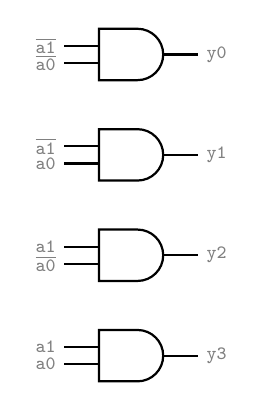
\begin{tikzpicture}[scale=0.85, transform shape]
      \foreach \y/\out/\la/\lb in {2.25/y0/$\overline{\ttab{a1}}$/$\overline{\ttab{a0}}$, 0.75/y1/$\overline{\ttab{a1}}$/\ttab{a0}, -0.75/y2/\ttab{a1}/$\overline{\ttab{a0}}$, -2.25/y3/\ttab{a1}/\ttab{a0}} {
        \node[and gate US, draw, thick, scale=1.3] (g) at (0,\y) {};
        \draw[thick] (g.input 1) -- ++(-0.5,0) node[left, smallgraytext] {\la};
        \draw[thick] (g.input 2) -- ++(-0.5,0) node[left, smallgraytext] {\lb};
        \draw[thick] (g.output) -- ++(0.5,0) node[right, smallgraytext] {\ttab{\out}};
      }
    \end{tikzpicture}
  \end{figure}
  \begin{center}
    \graytext{the address bits and their negations feed the gates}
  \end{center}
\end{frame}

% ------------------------------------------------------------
% encoder
% ------------------------------------------------------------
\begin{frame}{Encoder}
  \begin{center}
    \Large \highlight{\textbf{encoder}}
  \end{center}
\end{frame}

\begin{frame}
  An \highlight{\textbf{encoder}} does the reverse of a decoder. Given a one-hot input, it outputs the number of the input that is \ttab{1}.\\[3mm]
  \begin{minipage}{0.45\textwidth}
    \centering
    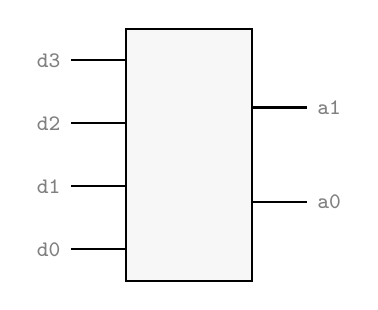
\begin{tikzpicture}
      \draw[thick, fill=gray!30!white!20] (0,-1.6) rectangle (1.6,1.6);
      \foreach \y/\l in {1.2/d3, 0.4/d2, -0.4/d1, -1.2/d0}
        \draw[thick] (0,\y) -- ++(-0.7,0) node[left, smallgraytext] {\ttab{\l}};
      \draw[thick] (1.6,0.6) -- ++(0.7,0) node[right, smallgraytext] {\ttab{a1}};
      \draw[thick] (1.6,-0.6) -- ++(0.7,0) node[right, smallgraytext] {\ttab{a0}};
    \end{tikzpicture}
  \end{minipage}%
  \begin{minipage}{0.55\textwidth}
    \centering
    \renewcommand{\arraystretch}{1.2}
    \begin{tabular}{cccc|cc}
      \ttab{d3} & \ttab{d2} & \ttab{d1} & \ttab{d0} & \ttab{a1} & \ttab{a0} \\ \hline
      \ttab{0} & \ttab{0} & \ttab{0} & \ttab{1} & \ttab{0} & \ttab{0} \\
      \ttab{0} & \ttab{0} & \ttab{1} & \ttab{0} & \ttab{0} & \ttab{1} \\
      \ttab{0} & \ttab{1} & \ttab{0} & \ttab{0} & \ttab{1} & \ttab{0} \\
      \ttab{1} & \ttab{0} & \ttab{0} & \ttab{0} & \ttab{1} & \ttab{1} \\
    \end{tabular}
  \end{minipage}
\end{frame}

% ------------------------------------------------------------
% don't-care values
% ------------------------------------------------------------
\begin{frame}{Don't-Care Values}
  \begin{center}
    \Large \highlight{\textbf{don't-care values}}
  \end{center}
\end{frame}

\begin{frame}
  Real devices, like a decoder for a digit display, have inputs that never occur. We mark their output as a \highlight{\textbf{don't-care}}, written \ttab{X}.\\[4mm]
  \begin{center}
    \renewcommand{\arraystretch}{1.2}
    \begin{tabular}{cc|c}
      \ttab{a1} & \ttab{a0} & \ttab{y} \\ \hline
      \ttab{0} & \ttab{0} & \ttab{1} \\
      \ttab{0} & \ttab{1} & \ttab{0} \\
      \ttab{1} & \ttab{0} & \ttab{X} \\
      \ttab{1} & \ttab{1} & \ttab{X} \\
    \end{tabular}
  \end{center}
    When we simplify, we may read each \ttab{X} as whichever value makes the groups larger. A don't-care is a free choice, used only when it helps.
\end{frame}

\end{document}